\documentclass{article}
\usepackage[utf8]{inputenc}
\usepackage{xcolor,listings}
\usepackage{textcomp}
\usepackage[utf8]{inputenc}
\usepackage{amsmath}
\usepackage{amssymb}
\usepackage{xcolor}
\usepackage{listings}
\usepackage{xstring}
\usepackage{graphicx}
\usepackage[export]{adjustbox}

\definecolor{dkgreen}{rgb}{0,0.6,0}
\definecolor{ltgray}{rgb}{0.5,0.5,0.5}

\makeatletter
\newif\ifcolname
\colnamefalse

\def\keywordcheck{%
\IfStrEq*{\the\lst@token}{select}{\global\colnametrue}{}%
\IfStrEq*{\the\lst@token}{where}{\global\colnametrue}{}%
\IfStrEq*{\the\lst@token}{from}{\global\colnamefalse}{}%
\color{blue}%
}
\def\setidcolor{%
\ifcolname\color{purple}\else\color{black}\fi%
}
\makeatother

\lstset{%
    backgroundcolor=\color{white},
    basicstyle=\footnotesize,
    breakatwhitespace=false,
    breaklines=true,
    captionpos=b,
    commentstyle=\color{dkgreen},
    deletekeywords={...},
    escapeinside={\%*}{*)},
    extendedchars=true,
    frame=single,
    keepspaces=true,
    language=SQL,
    otherkeywords={is},
    morekeywords={*,modify,MODIFY,...},
    keywordstyle=\keywordcheck,
    identifierstyle=\setidcolor,
    numbers=left,
    numbersep=15pt,
    numberstyle=\tiny,
    rulecolor=\color{ltgray},
    showspaces=false,
    showstringspaces=false, 
    showtabs=false,
    stepnumber=1,
    tabsize=4,
    title=\lstname
}
\lstset{upquote=true}
\renewcommand\thesubsection{\alph{subsection}}
\usepackage{graphicx}
\title{CS313, Assignment - 2}
\author{Shashank P, 200010048}
\date{\today}

\begin{document}

\maketitle

\section{Integrity Constraints in Univeristy Table}

    \begin{table}[ht]
\begin{tabular}{||p{2cm}||p{2cm}||p{2cm}||p{3cm}||p{2cm}||}
\hline  
\hline
\textbf{Table} & \textbf{Primary Key}  & \textbf{Domain of PK} & \textbf{Foreign key(Referencing
table)} & \textbf{Not Null}\\
 \hline \hline
 
classroom & building, room\_number  & varchar & - & building, room\_number \\ \hline \hline
department & dept\_name  & varchar & - & dept\_name \\ \hline \hline

course & course\_id  & varchar & foreign key (dept\_name) \newline references \newline department & course\_id \\ \hline

instructor & ID  & varchar & foreign key (dept\_name) \newline references \newline department & name, ID \\ \hline

section & course\_id, sec\_id, semester, year & varchar \newline varchar \newline varchar \newline numeric & foreign key (course\_id) \newline references course, \newline 
	 foreign key (building, room\_number) references classroom & course\_id, sec\_id, semester, year \\ \hline \hline
	 
teaches & ID, course\_id, sec\_id, semester, year & varchar \newline varchar \newline varchar \newline varchar \newline numeric \newline & foreign key (course\_id,sec\_id, semester, year) references \newline section,
	 foreign key (ID) references instructor & ID, course\_id, sec\_id, semester, year\\ \hline \hline
	 

\end{tabular}
\end{table}

\clearpage

    \begin{table}[ht]
\begin{tabular}{||p{2cm}||p{2cm}||p{2cm}||p{3cm}||p{2cm}||}
\hline \hline
 
student & ID & varchar & foreign key (dept\_name) references department & ID, name \\ \hline \hline

takes & ID, course\_id, sec\_id, semester, year & varchar \newline varchar \newline varchar \newline varchar \newline numeric & foreign key (course\_id,sec\_id, semester, year) references section,
	 foreign key (ID) references student & ID, course\_id, sec\_id, semester, year \\ \hline \hline

advisor & s\_ID  & varchar & foreign key (i\_ID) references instructor (ID), foreign key (s\_ID) references student (ID) & s\_ID \\ \hline \hline

time\_slot & time\_slot\_id, day, start\_hr, start\_min & varchar \newline varchar \newline numeric \newline numeric & - & time\_slot\_id, day, start\_hr, start\_min \\ \hline \hline
	 
prereq & course\_id, prereq\_id & varchar \newline varchar & foreign key (course\_id) references course,
	 foreign key (prereq\_id) references course & course\_id, prereq\_id\\ \hline \hline
	 

\end{tabular}
\caption{Integrity Constraints of all tables}
\end{table}

\newpage
\section{One student's complete profile}
Select complete profile of a student named 'Shankar' from multiple tables.
\begin{lstlisting}[language=sql]
select * from student, department, takes, advisor, instructor
where student.name='Shankar' 
  and student.dept_name=department.dept_name 
  and student.ID=takes.ID 
  and (student.ID=advisor.s_ID and instructor.ID=advisor.i_ID) 
  and department.dept_name=instructor.dept_name;
\end{lstlisting}

\begin{figure}[!ht]
  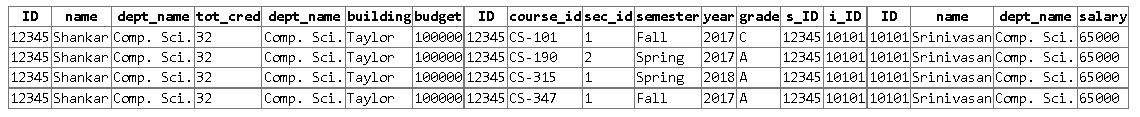
\includegraphics[scale=0.61]{4.png}
  \caption{Query output}
\end{figure}




\section{Trying out various queries}

\subsection{Table: classroom}
\begin{lstlisting}[language=sql]
  insert into classroom values('My Building', 1234, 1000);
  select building, room_number from classroom where capacity>=50;
\end{lstlisting}
\begin{figure}[!ht]
  \begin{center}
  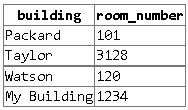
\includegraphics[scale=1]{class.png}
  \caption{Query output}
  \end{center}
\end{figure}

\subsection{Table: department}
\begin{lstlisting}[language=sql]
  insert into department values('My New Department', 'Watson', 200000);
  select * from department where budget between 50000 and 210000;
\end{lstlisting}
\begin{figure}[!ht]
  \begin{center}
  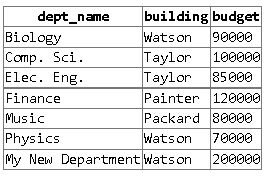
\includegraphics[scale=1]{dep.png}
  \caption{Query output}
  \end{center}
\end{figure}

\subsection{Table: course}
\begin{lstlisting}[language=sql]
  insert into course values('NN-101', 'A New Course', 'History', 5);
  select max(credits) from course;
\end{lstlisting}
\begin{figure}[!ht]
  \begin{center}
  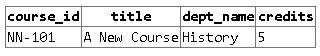
\includegraphics[scale=1]{course.png}
  \caption{Query output}
  \end{center}
\end{figure}

\subsection{Table: instructor}
\begin{lstlisting}[language=sql]
  insert into instructor values('12345', 'A New Instructor', 'Comp. Sci.', 50000);
  select ID, name from instructor where dept_name in ('Comp. Sci.', "Physics");
\end{lstlisting}
\begin{figure}[!ht]
  \begin{center}
  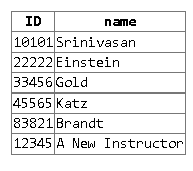
\includegraphics[scale=0.75]{inst.png}
  \caption{Query output}
  \end{center}
\end{figure}

\newpage
\subsection{Table: section}
\begin{lstlisting}[language=sql]
  insert into section values('CS-319', '3', 'Summer', 2019, 'Watson', '514', 'A');
  select * from section where course_id='CS-319' order by time_slot_id asc
\end{lstlisting}
\begin{figure}[!ht]
  \begin{center}
  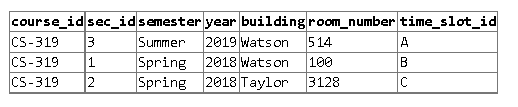
\includegraphics[scale=1]{sec.png}
  \caption{Query output}
  \end{center}
\end{figure}

\subsection{Table: teaches}
\begin{lstlisting}[language=sql]
  insert into teaches values('45565', 'CS-101', '1', 'Fall', 2016);
  select max(year), min(year) from teaches where ID='45565';
\end{lstlisting}
\begin{figure}[!ht]
  \begin{center}
  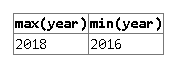
\includegraphics[scale=1]{teaches.png}
  \caption{Query output}
  \end{center}
\end{figure}

\subsection{Table: student}
\begin{lstlisting}[language=sql]
  insert into student values('99999', 'New Name', 'Comp. Sci.', 250);
  select ID, name from student where tot_cred in (select max(tot_cred) from student);
\end{lstlisting}
\begin{figure}[!ht]
  \begin{center}
  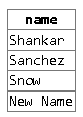
\includegraphics[scale=1]{student.png}
  \caption{Query output}
  \end{center}
\end{figure}

\subsection{Table: takes}
\begin{lstlisting}[language=sql]
  insert into takes values('44553', 'CS-347', '1', 'Fall', 2017, 'A-');
  select * from takes where ID=='44553';
\end{lstlisting}
\begin{figure}[!ht]
  \begin{center}
  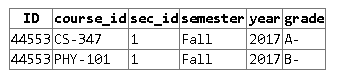
\includegraphics[scale=1]{takes.png}
  \caption{Query output}
  \end{center}
\end{figure}

\newpage
\subsection{Table: advisor}
\begin{lstlisting}[language=sql]
  insert into advisor values('19991', '22222');
  select * from advisor where i_ID='22222';
\end{lstlisting}
\begin{figure}[!ht]
  \begin{center}
  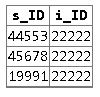
\includegraphics[scale=1]{adv.png}
  \caption{Query output}
  \end{center}
\end{figure}

\subsection{Table: time\_slot}
\begin{lstlisting}[language=sql]
  insert into time_slot values('NEW', 'R', 13, 31, 14, 45);
  select * from time_slot where day='R';
\end{lstlisting}
\begin{figure}[!ht]
  \begin{center}
  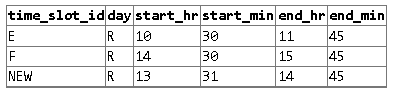
\includegraphics[scale=1]{time_slot.png}
  \caption{Query output}
  \end{center}
\end{figure}

\subsection{Table: prereq}
\begin{lstlisting}[language=sql]
  insert into prereq values('PHY-101', 'BIO-101');
  select * from prereq where prereq_id='BIO-101';
\end{lstlisting}
\begin{figure}[!ht]
  \begin{center}
  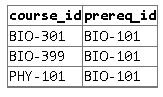
\includegraphics[scale=1]{ew.png}
  \caption{Query output}
  \end{center}
\end{figure}

\newpage
\section{Additional Queries}
\subsection{Stduent taking Comp. Sci. from Watson building}
\begin{lstlisting}[language=sql]
  select student.ID, student.name from student, takes, section 
  where student.dept_name='Comp. Sci.' 
    and student.ID=takes.ID 
    and takes.course_id=section.course_id 
    and section.building='Watson'
\end{lstlisting}
\begin{figure}[!ht]
  \begin{center}
  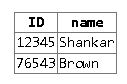
\includegraphics[scale=1]{4_a.png}
  \caption{Query output}
  \end{center}
\end{figure}

\subsection{Student having both 'A' and 'C' grade}
\begin{lstlisting}[language=sql]
select ID, name 
from student natural join takes 
where takes.grade='A'

intersect

select ID, name 
from student natural join takes 
where takes.grade='C'
\end{lstlisting}
\begin{figure}[!ht]
  \begin{center}
  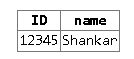
\includegraphics[scale=1]{4_b.png}
  \caption{Query output}
  \end{center}
\end{figure}
\newpage
\subsection{Buildings that have classes on Wednesday}
\begin{lstlisting}[language=sql]
  select distinct building, room_number
  from section natural join time_slot
  where time_slot.day='W'
\end{lstlisting}
\begin{figure}[!ht]
  \begin{center}
  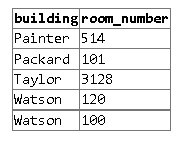
\includegraphics[scale=1]{4_c.png}
  \caption{Query output}
  \end{center}
\end{figure}


\end{document}